
\section{Barrier Certificate Search for Second Order 1D System}\label{sec:sos_2ndorder_error}
Now a second order model of the robot slide position is used in the search for a barrier certificate for the 1D system, with the system model as found in \autoref{subsec:model_2d}
\begin{equation}
\dot{\mathbf{x}}= 
\begin{bmatrix}
0 & 1\\
-\omega_n^2  & -2\zeta \omega_n  
\end{bmatrix}
\mathbf{x} + 
\begin{bmatrix}
0\\\omega_n^2
\end{bmatrix}\left(\bar{\mathbf{N}}x_\text{ref}-\mathbf{K}\mathbf{x}\right),
 \kk \text{with }
 \omega_n = 17 \,\text{rad/s}, \quad \zeta = 0.55
\end{equation}
where again the matrix $\bar{\mathbf{N}}$ ensures unity gain between the position and its reference, which means that $\bar{\mathbf{N}}=K_1+1$. Now the position error is 
\begin{align*}
x_\text{err,1}&=x_\text{ref}-x_1\\
\dot{x}_\text{err,1} &= -\dot{x}_1 \,=-x_2=x_\text{err,2}\\
\ddot{x}_\text{err,1} &= \dot{x}_\text{err,2} = -\dot{x}_2 = \omega_n^2 x_1 +2\zeta\omega_n x_2 - \omega_n^2(\bar{\mathbf{N}}x_\text{ref}-(K_1x_1+K_2 x_2))\nonumber\\
& \phantom{= -\ddot{x}_\text{err,1} = \dot{x}_2. } = (2\zeta\omega_n +K_2)x_2 -\omega_n^2(K_1+1)(x_\text{ref}-x_1)\nonumber\\
& \phantom{= -\ddot{x}_\text{err,1} = \dot{x}_2. } = -(2\zeta\omega_n +K_2){x}_\text{err,2} - \omega_n^2(K_1+1)x_\text{err,1}
%- 5.173\dot{x}_1(t)  -  0.214\dot{x}_2(t) &= -5.173x_2 -0.214(- \omega_n^2 x_1 - 2\zeta \omega_n x_2 + \omega_n^2 x_\text{err} )\nonumber\\
%&= (0.214\cdot2\zeta \omega_n - 5.173)x_2 + 0.214\omega_n^2\underbrace{(x_1-x_\text{err})}_{\textcolor{red}{x_\text{ref} ???}}
\end{align*}
giving the error state-space equation
\begin{equation}
\dot{\mathbf{x}}_\text{err}= 
\dot{\begin{bmatrix}
{x}_\text{err,1} \\ 
{x}_\text{err,2}
\end{bmatrix}} =
\begin{bmatrix}
0 & 1 \\
-\omega_n^2(K_1+1) & -(2\zeta\omega_n +K_2)
\end{bmatrix}
\begin{bmatrix}
x_\text{err,1} \\ {x}_\text{err,2}
\end{bmatrix}
\end{equation}

As for the first order system, the unsafe set is $\mathcal{X}_u=\{x_1\in[0.05,0.1] \}$, and it is assumed that references are never given in the unsafe set (or outside the physical limits of the slide position). Hence it is again the goal to limit the position error in negative direction (tool position above reference), while the velocity of the error obviously has the same physical limits as the velocity of the robot tool, i.e. a maximum velocity of $\pm 0.5$\,m/s. This means that the sets are defined as $\mathcal{X}=\{x_\text{err,1}\in[-0.03,0.03], x_\text{err,2}\in[-1,1] \}$, the unsafe set $\mathcal{X}_u=\{x_\text{err,1}\in[-0.03,-\delta_\text{err}], x_\text{err,2}\in[-1,1] \}$ and the safe set $\mathcal{X}_0=\{x_\text{err,1}\in[-\delta_\text{err} +\Delta,0.03], x_\text{err,2}\in[-1,1] \}$, see \autoref{fig:sos_error_2d_2ndorder}, and it is again desired to find as small a value $\delta_\text{err}$ as possible, thus guaranteeing system safety for references until a minimum distance $\delta_\text{err}$ from the region of unsafe positions, see \autoref{fig:sos_error_1d_2ndorder} and \ref{fig:sos_errorref_1d_2ndorder}.

\begin{figure}[H]
	\centering
	\subbottom[]{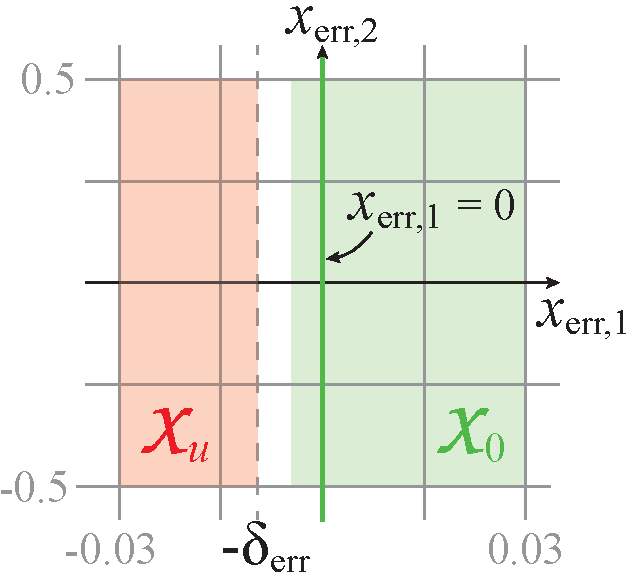
\includegraphics[width=0.3\textwidth]{sos_error_2d_2ndorder.pdf}\label{fig:sos_error_2d_2ndorder}}%
	\hspace{3mm}
	\subbottom[]{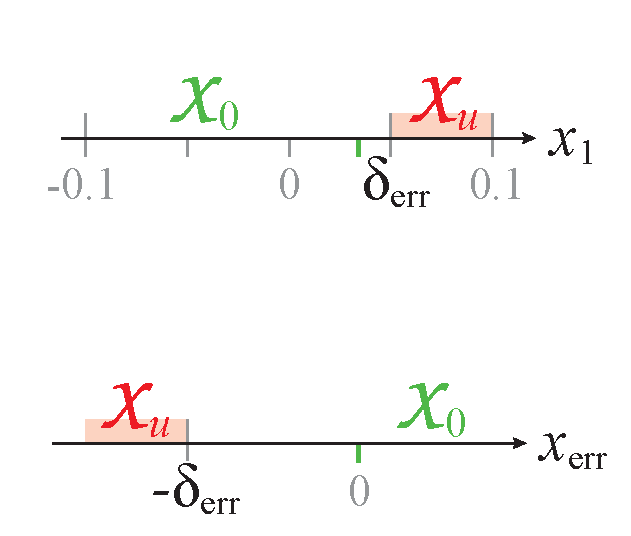
\includegraphics[width=0.3\textwidth]{sos_error_1d.pdf}\label{fig:sos_error_1d_2ndorder}}%
	\hspace{3mm}
	\subbottom[]{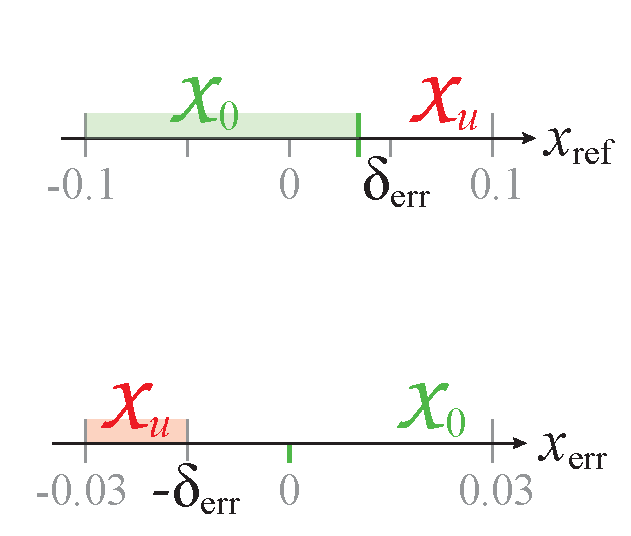
\includegraphics[width=0.3\textwidth]{sos_errorref_1d.pdf}\label{fig:sos_errorref_1d_2ndorder}}%
	\caption{With references given outside the unsafe region, system safety can be guaranteed if the error is certified to stay above the value $-\delta_\text{err}$. When this is the case, system safety is guaranteed for all references up to a safety distance of $\delta_\text{err}$ from the unsafe set.}
	\label{fig:sets_error_2ndorder}
\end{figure}

Again, the same parameters as in \autoref{sec:sos_1storder_references} and \ref{sec:sos_1storder_error} are varied, and the same conclusions are drawn i.e. in general decreasing either  $\Delta$, $\bar{\epsilon}$ or deg$(q)$ decreases the residual norm. With  $\textbf{K}=[5.173  \,\,\,\,  0.214]$ as determined in \autoref{eq:K_2}, solutions can be found to the problem for $\delta_\text{err}=8$\,mm and above, again signifying a verification that the system is safe for references given at a distance of least 8\,mm from the unsafe area.

\begin{figure}[H]
	\centering
	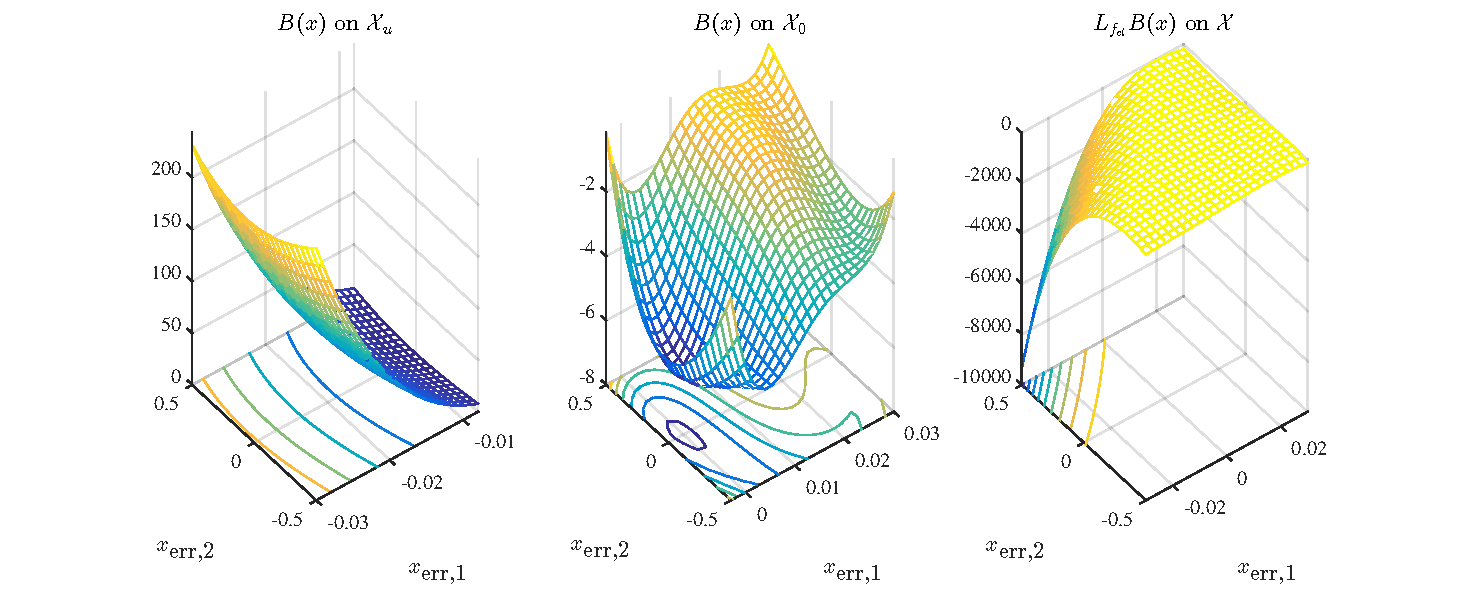
\includegraphics[width=\textwidth]{1D_2ndordersys_error_B4_q1_e5-2_d5-3_8mm.pdf}
	\caption{Barrier certificate of degree [0:4], all \gls{sos} polynomials of degree [0:1], $\bar{\epsilon}=5$e-2, $\Delta=5$\,mm and $\delta_\text{err}=8$\,mm gives \texttt{feasratio=1.0176} and \texttt{Residual norm=3.2e-6}.}
	\label{fig:1D_2ndordersys_error_B4_q1_e5-2_d5-3_8mm}
\end{figure}

\begin{figure}[H]
	\centering
	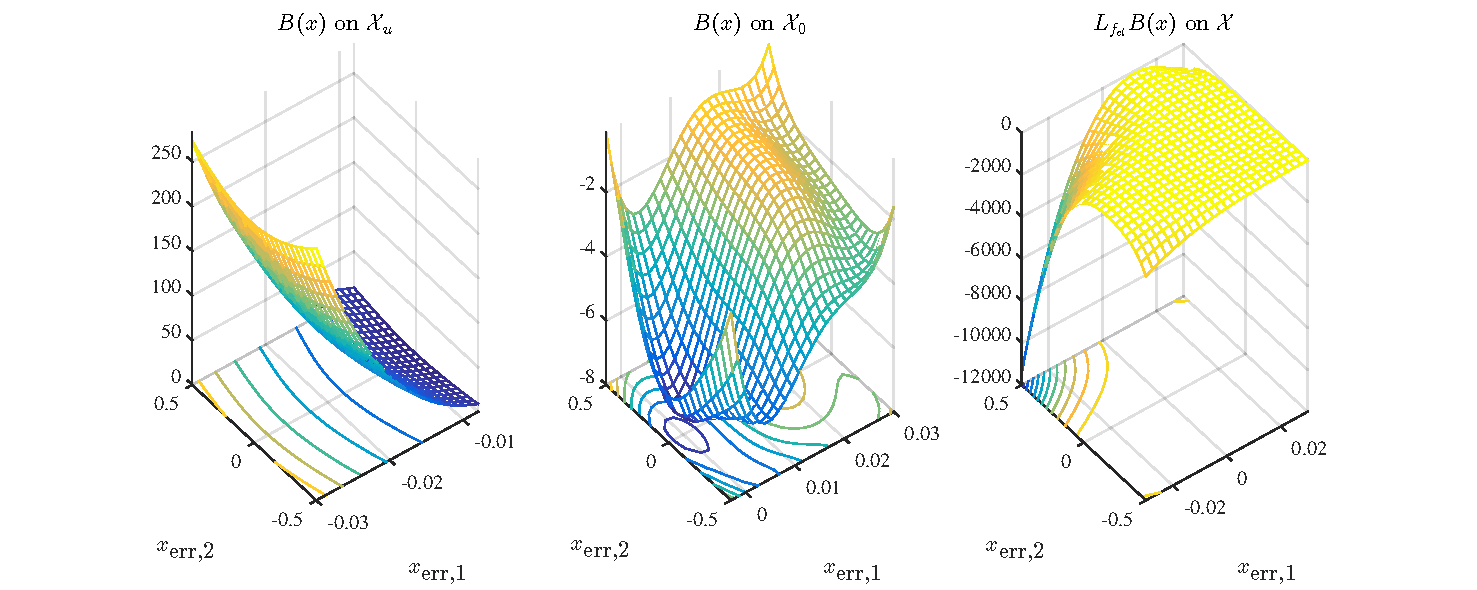
\includegraphics[width=\textwidth]{1D_2ndordersys_error_B6_q2_e5-2_d5-3_8mm.pdf}
	\caption{Barrier certificate of degree [0:6], all \gls{sos} polynomials of degree [0:2], $\bar{\epsilon}=5$e-2, $\Delta=5$\,mm and $\delta_\text{err}=8$\,mm gives \texttt{feasratio=0.9500} and \texttt{Residual norm=1.8e-5}.}
	\label{fig:1D_2ndordersys_error_B6_q2_e5-2_d5-3_8mm}
\end{figure}

\begin{figure}[H]
	\centering
	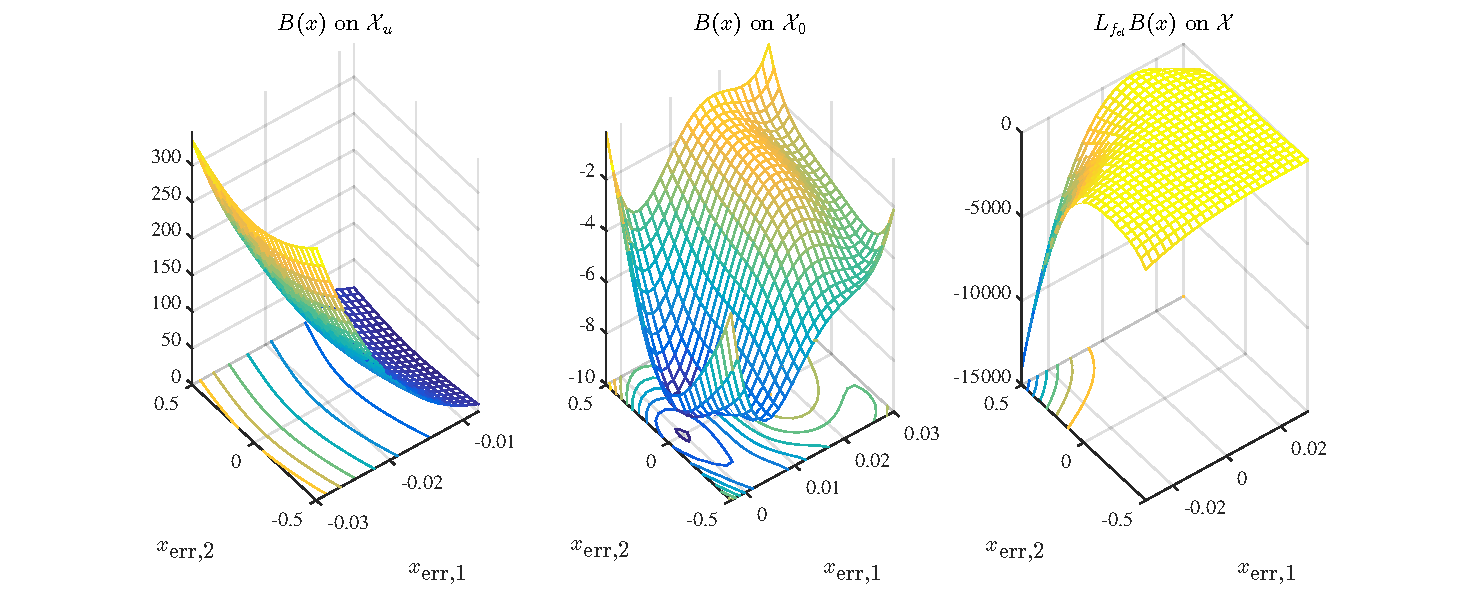
\includegraphics[width=\textwidth]{1D_2ndordersys_error_B8_q3_e5-2_d5-3_8mm.pdf}
	\caption{Barrier certificate of degree [0:8], all \gls{sos} polynomials of degree [0:3], $\bar{\epsilon}=5$e-2, $\Delta=5$\,mm and $\delta_\text{err}=8$\,mm gives \texttt{feasratio=0.9882} and \texttt{Residual norm=4.5e-5}.}
	\label{fig:1D_2ndordersys_error_B8_q3_e5-2_d5-3_8mm}
\end{figure}

Three examples of solutions are seen in \autoref{fig:1D_2ndordersys_error_B4_q1_e5-2_d5-3_8mm}, \ref{fig:1D_2ndordersys_error_B6_q2_e5-2_d5-3_8mm} and \ref{fig:1D_2ndordersys_error_B8_q3_e5-2_d5-3_8mm} with $\delta_\text{err}=8$\,mm and with a minimum value in the unsafe set $\bar{\epsilon}=5$e-2. Compared to the first order system increasing the degrees of the barrier function and the \gls{sos} polynomials  more clearly causes a scaling of the functional values, while the curves are close to identical in shape on the sets. The residual norm of the solution is growing when the polynomial degrees are increased, confirming the intuition that it is preferred to keep the polynomial degrees as low as possible. Numerical problems are reported for all three solutions as for almost all solutions found, however, numerical errors are only indicated for the two lowest-order polynomials plotted in \autoref{fig:1D_2ndordersys_error_B4_q1_e5-2_d5-3_8mm} and \ref{fig:1D_2ndordersys_error_B6_q2_e5-2_d5-3_8mm}, but not for the solution plotted in \autoref{fig:1D_2ndordersys_error_B8_q3_e5-2_d5-3_8mm}.

%From \autoref{eq:K_2}
%\begin{flalign}
%	\mathbf{K} = \texttt{acker(A,B,C,D,[-40 -50])} = \begin{bmatrix}
%		5.173  &  0.214
%	\end{bmatrix}
%\end{flalign}

%From \autoref{eq:Nbar_2}
%\begin{flalign}
%	\bar{\mathbf{N}} = - \left( \mathbf{C}\,\mathbf{A}_{cl}^{-1}\,\mathbf{B} \right)^{-1} =  - \left( \mathbf{C}\,(\mathbf{A}-\mathbf{B}\,\mathbf{K})^{-1}\,\mathbf{B} \right)^{-1} = 6.173
%\end{flalign}